\thispagestyle{duongvaotoanhocnone}
\pagestyle{duongvaotoanhoc}
\everymath{\color{duongvaotoanhoc}}
\graphicspath{{../duongvaotoanhoc/pic2/}}
\blfootnote{$^*$\color{duongvaotoanhoc}Nguồn: https://www.quantamagazine.org/hobbyist-finds-maths-elusive-einstein-tile-20230404.}
\blfootnote{\color{duongvaotoanhoc}$^1$THPT chuyên Hà Nội -- Amsterdam }
\begingroup
\AddToShipoutPicture*{\put(0,616){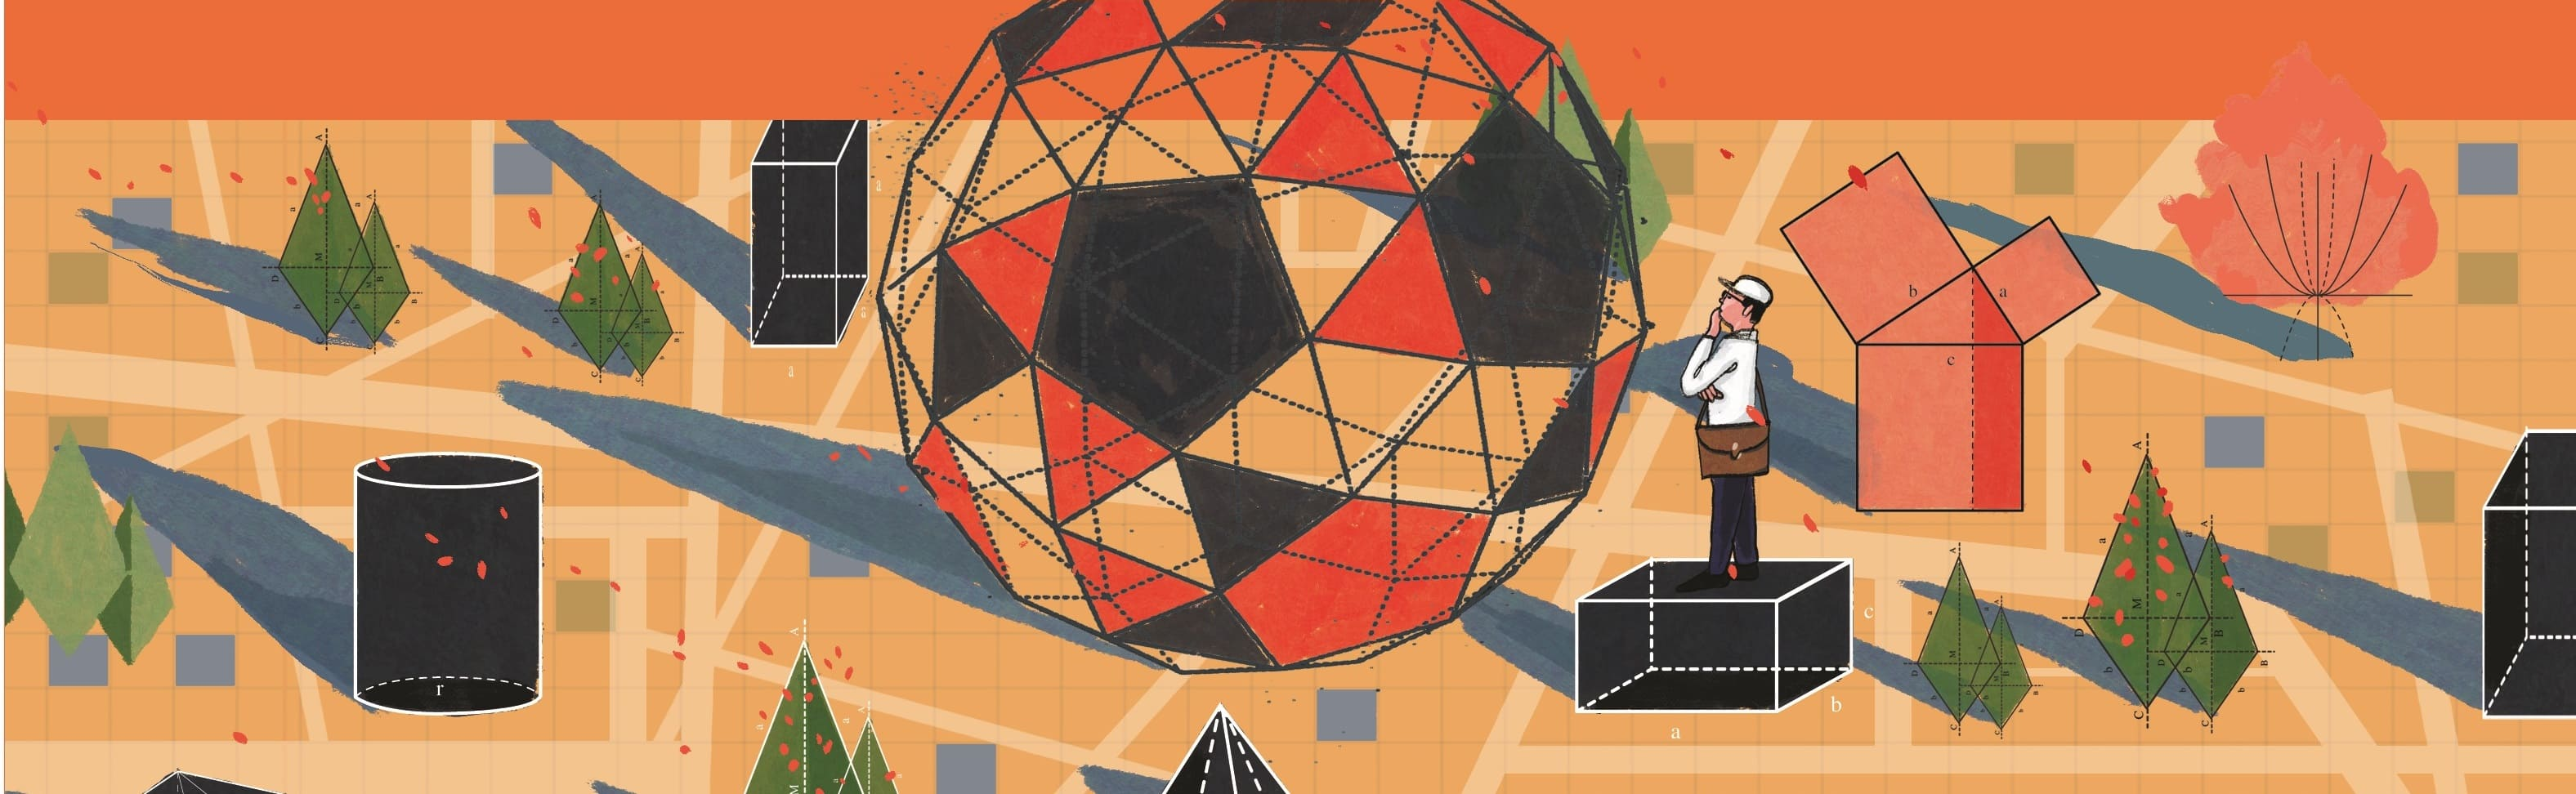
\includegraphics[width=19.3cm]{../bannerduongvao}}}
\AddToShipoutPicture*{\put(76,500){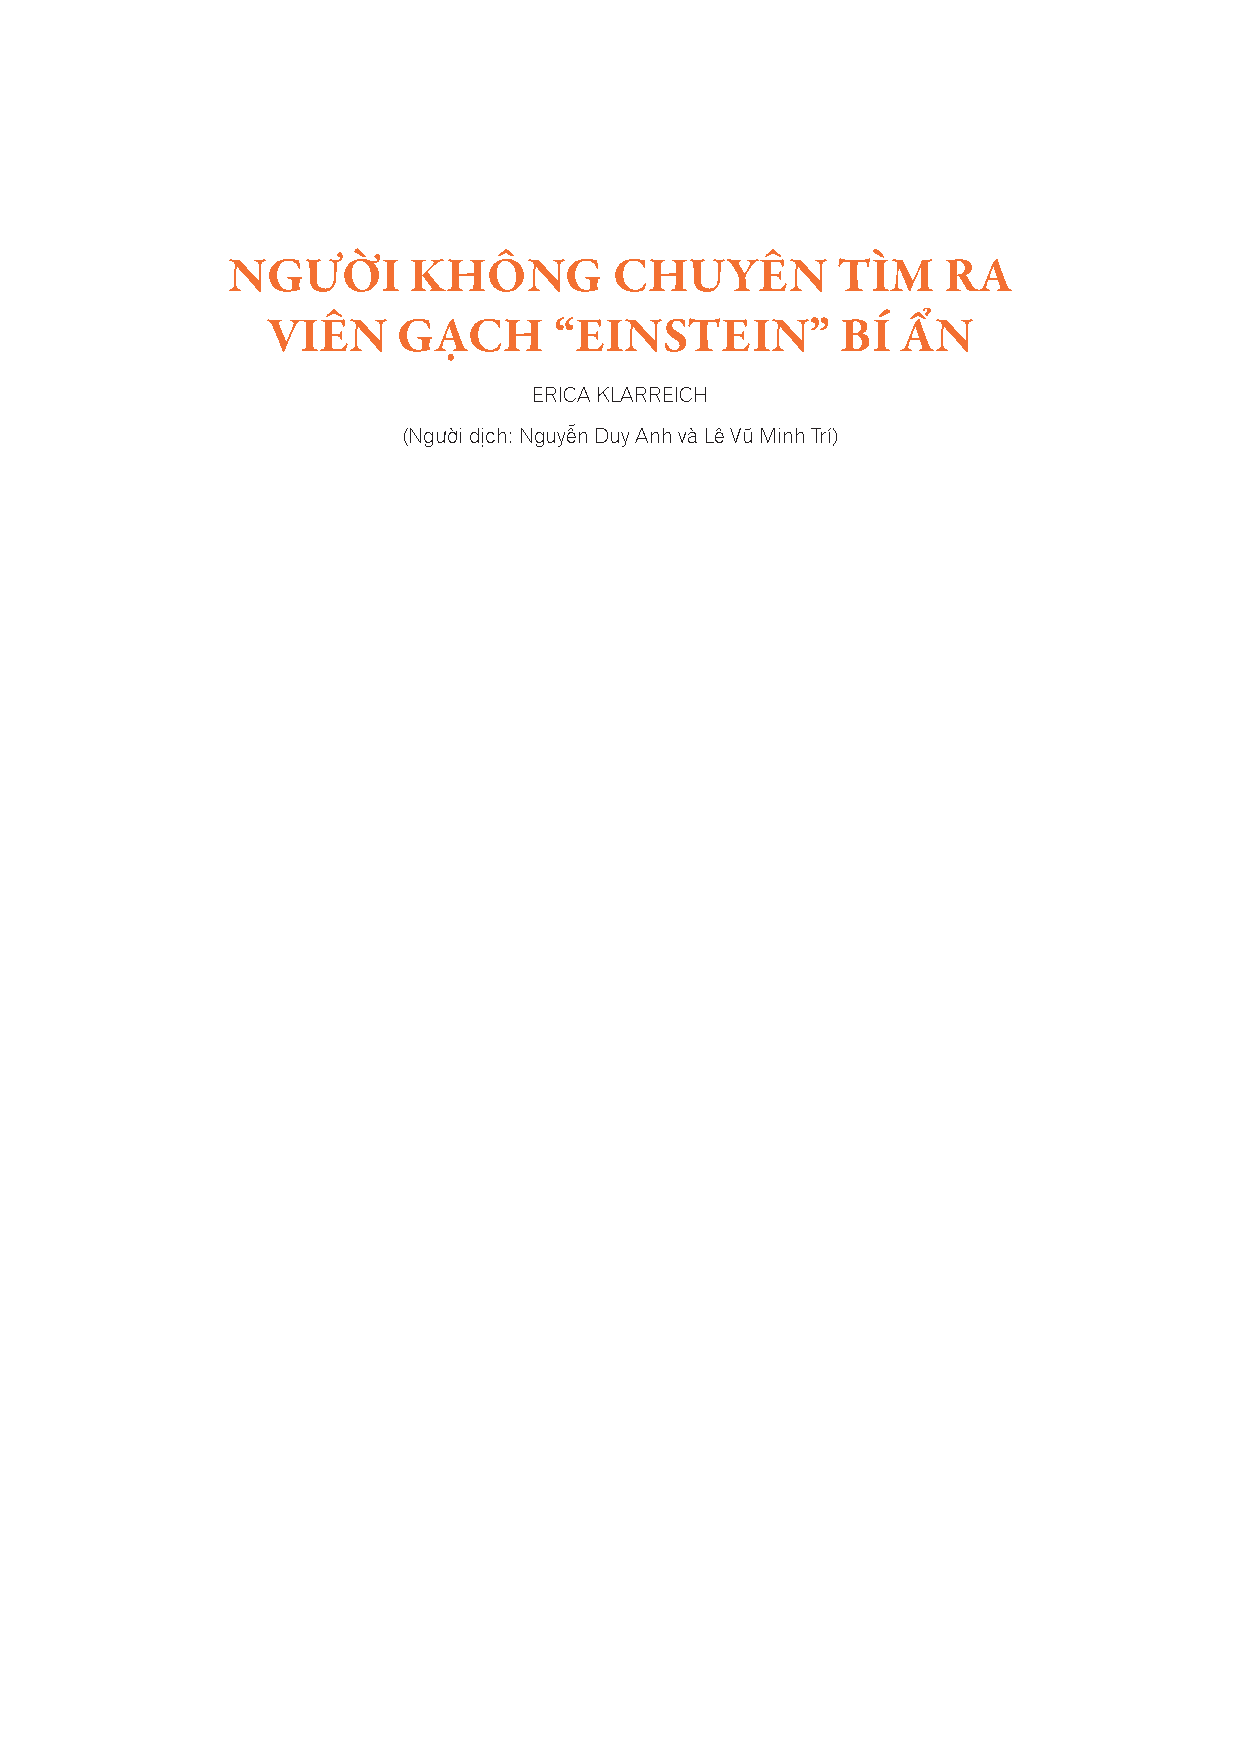
\includegraphics[scale=1]{../tieude1.pdf}}}
\centering
\endgroup
\vspace*{208pt}

\begin{multicols}{2}	
	Giữa tháng $11$ năm $2022$, David Smith [$1$], một kỹ thuật viên in ấn đã nghỉ hưu có niềm vui thú với xếp hình, hình học fractal và bản đồ đường xá, đang làm việc mình yêu thích: chơi với những hình khối. Nhờ một phần mềm gọi là ``PolyForm Puzzle Solver" [$2$], ông đã dựng được một miếng gạch hình cái mũ trông khá khiêm tốn. Ông đã bắt đầu thử nghiệm xem có thể phủ kín được bao nhiêu phần màn hình với duy nhất viên gạch lát này, với điều kiện không để hai viên đè lên nhau hay để hở khoảng trống.
	\vskip 0.1cm
	Thường thì khi ông tạo ra loại gạch mới, chúng sẽ hoặc tạo thành một họa tiết lặp, hoặc chỉ lát được một phần nhỏ màn hình. Viên gạch mũ có vẻ không thuộc cả hai loại này. Thế là Smith cắt $30$ miếng giấy bìa màu hình viên gạch này và xếp chúng trên bàn. Rồi ông cắt thêm $30$ cái nữa và tiếp tục xếp. ``Tôi dần nhận ra rằng mỗi lần xếp là một cách lát tôi chưa thấy bao giờ," ông nói. ``Đó là một viên gạch lát ranh mãnh". Ông gửi mô tả về viên gạch tới Craig Kaplan [$3$], một nhà khoa học máy tính ông quen tại Đại học Waterloo, Canada. Kaplan ngay lập tức bắt đầu tìm hiểu các tính chất của nó.
	\vskip 0.1cm
	Ngày $20$ tháng $3$ vừa qua, Smith và Kaplan, cùng với $2$ nhà nghiên cứu nữa, đã công bố [$4$] rằng đây chính là thứ mà các nhà toán học đã tìm kiếm suốt hơn năm thập kỉ: một viên gạch duy nhất mà ta có thể dùng để lát toàn mặt phẳng, nhưng chỉ theo những họa tiết không lặp lại bất kỳ khối gạch nào. Các nhà toán học gọi những viên gạch, hoặc các bộ viên gạch, có tính chất đó là ``phi tuần hoàn" (aperiodic), trái với hình vuông hoặc lục giác là những hình có thể phủ cả mặt phẳng theo các họa tiết lặp lại (hay ``tuần hoàn").
	\vskip 0.1cm
	Viên gạch mũ ẩn chứa ``đủ sự phức tạp để bẻ gãy trật tự tuần hoàn theo mọi quy mô", các nhà nghiên cứu khẳng định trong bài báo. Hơn nữa, họ nhận ra rằng viên gạch mũ là một trong vô số viên gạch khác nhau có cùng tính chất này.
	\vskip 0.1cm
	``Tưởng xa tận chân trời mà gần ngay trước mắt,"  là những gì  Doris Schattschneider, giáo sư toán danh dự tại Đại học Moravian, Pennsylvania nói về viên gạch này.  Bà tả rằng bản thân đã ``sửng sốt" trước phát hiện này.
	\vskip 0.1cm
	Các nhà toán học đã bắt đầu tìm kiếm một viên gạch như viên gạch mũ từ những năm 60 thế kỷ trước, khi Robert Berger  [$5$] dựng ra $20426$ loại gạch cùng nhau lát mặt phẳng một cách phi tuần hoàn. Công trình này là phát súng mở màn cho một cuộc đua dựng ra các bộ gạch có thể lát mặt phẳng phi tuần hoàn bằng ít loại hơn, lên đến đỉnh điểm là khám phá của Roger Penrose vào thập niên $70$ với chỉ hai viên. Năm $1982$, Dan Shechtman [$6$] đã tìm ra những dạng đối xứng tương tự như của gạch lát Penrose trong tự nhiên, dưới hình hài các cấu trúc gọi là giả tinh thể (quasicrystal), qua đó giúp ông đạt giải Nobel Hóa học năm $2011$.
	\begin{figure}[H]
		\vspace*{-5pt}
		\centering
		\captionsetup{labelformat= empty, justification=centering}
		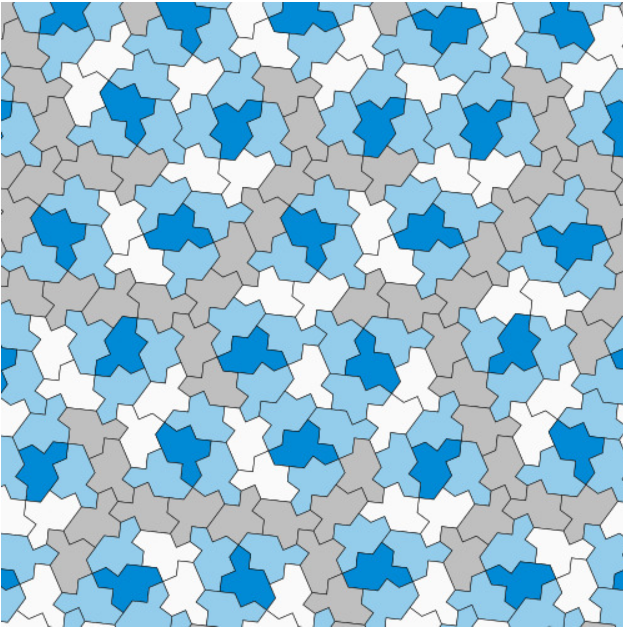
\includegraphics[width= 1\linewidth]{1}
		\caption{\small\textit{\color{duongvaotoanhoc}Viên gạch mũ chỉ là một trong một họ các viên gạch phi tuần hoàn}}
		\vspace*{-10pt}
	\end{figure}
	Từ ấy, các nhà toán học vẫn không ngừng tìm kiếm một loại gạch duy nhất có thể lát mặt phẳng $2$ chiều một cách phi tuần hoàn, mà không cho phép kẽ hở hay gạch đè lên nhau. Ludwig Danzer, một nhà hình học người Đức, đã tinh nghịch đặt tên cho loại gạch như thế là một ``einstein" -- chơi chữ của cụm từ tiếng Đức ``ein stein", nghĩa là ``một miếng".
	\vskip 0.1cm
	Vào những năm $1990$, hai nhóm khác nhau  [$7$] đã tìm ra cách chồng kề nhau một loại gạch $10$ cạnh để phủ mặt phẳng. Trong thập kỷ sau đó, Joan Taylor [$8$], một nhà toán học nghiệp dư ở Tasmania, đã khám phá ra một hình với nhiều miếng không liền  với nhau  [$9$]. Cùng với Joshua Socolar [$10$], một nhà vật lý tại Đại học Duke, họ đã chứng minh được hình này có thể lát mặt phẳng một cách phi tuần hoàn  [$11$]. Và mới năm ngoái, Rachel Greenfield [$12$] từ Viện Nghiên cứu Cao cấp Princeton và Terence Tao [$13$] từ Đại học California, Los Angeles đã phát hiện ra một hình trong không gian nhiều chiều [$14$] có thể lát không gian một cách phi tuần hoàn mà không cần quay hay lật.
	\vskip 0.1cm
	Nhưng chưa ai tìm được một ``einstein" đích thực -- một hình $2$ chiều đơn giản phủ mặt phẳng một cách phi tuần hoàn. Cuối cùng, giới toán học bắt đầu nghi ngờ sự tồn tại của chúng, theo lời Marjorie Senechal [$15$], một nhà nghiên cứu về lát gạch và giáo sư danh dự tại Đại học Smith. Bà cho biết thêm: việc một ``einstein" đơn giản như viên gạch mũ của Smith lù lù trước mắt, chờ đợi được tìm ra là một sự thật ``khó tin". 
	\vskip 0.1cm
	Theo bà phỏng đoán, có lẽ lý do viên gạch mũ tránh được sự tìm kiếm đến tận bây giờ là do nhiều nhà toán học đã tập trung vào các hình đối xứng kiểu ``cấm kỵ" -- những kiểu mà không thể có trong các loại gạch lát tuần hoàn. Chẳng hạn như gạch lát Penrose có ``đối xứng gấp $5$" (đối xứng qua phép quay $72$ độ quanh tâm), như ở các ngũ giác đều hay hình ngôi sao. Các ngũ giác đều không thể phủ mặt phẳng, nên bắt đầu từ các ``đối xứng gấp $5$" là khởi điểm khá tự nhiên. 
	\vskip 0.1cm
	Trái lại, viên gạch mũ chẳng có đối xứng nào cả, và ``đơn giản đến mức tầm thường", các tác giả bình luận. Cách lát này có quan hệ mật thiết với một cách lát tuần hoàn: lưới tổ ong hình lục giác. Ta có thể tạo ra cách lát hình mũ từ cách lát bằng lục giác như sau: trước hết nối các trung điểm các cặp cạnh đối của lục giác. Lục giác sẽ bị chia thành 6 hình ``cánh diều". Mỗi viên gạch mũ được cấu thành từ $8$ hình cánh diều liền nhau, kết hợp từ các lục giác kề nhau. Bất kỳ ai đầu tư chút sức lực, cùng một cái bút dạ và sàn nhà vệ sinh gạch hình lục giác cũng có thể viền được một cách phủ mặt phẳng bằng hình mũ.  
	\begin{figure}[H]
		\vspace*{-5pt}
		\centering
		\captionsetup{labelformat= empty, justification=centering}
		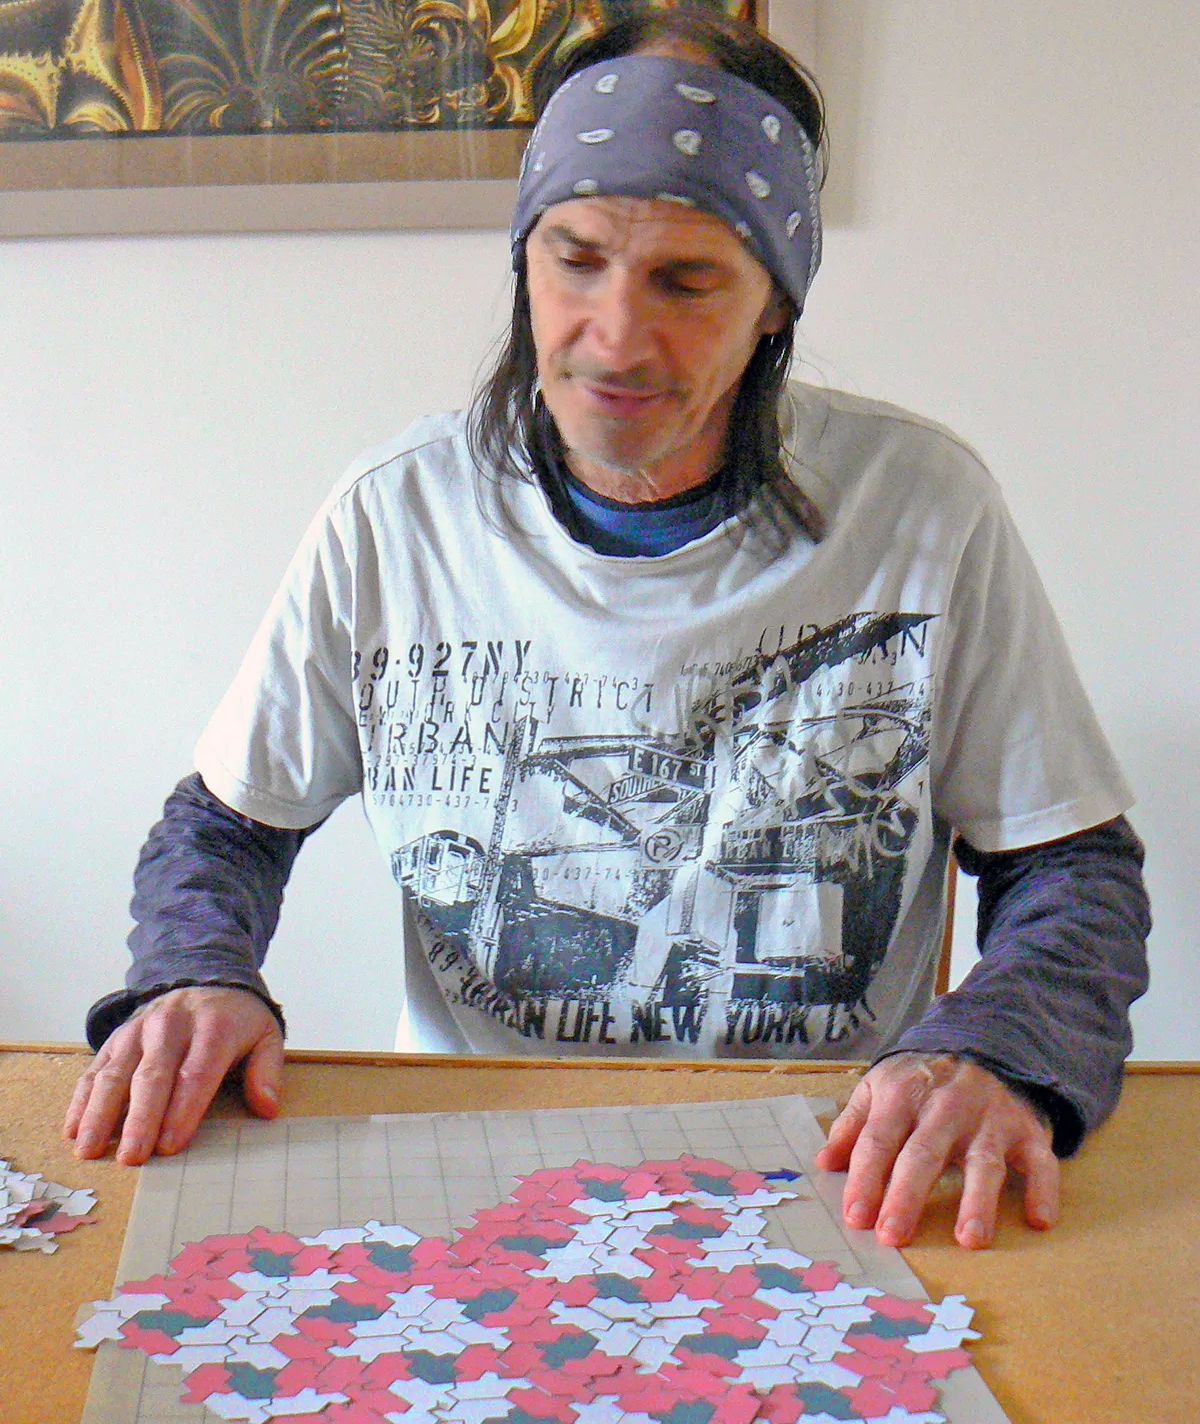
\includegraphics[width= 1\linewidth]{2}
		\caption{\small\textit{\color{duongvaotoanhoc}Khám phá của David Smith được coi là một khám phá khó tin.}}
		\vspace*{-10pt}
	\end{figure}
	Viên gạch mũ, Senechal nói, chỉ ra rằng sự liên kết giữa gạch lát tuần hoàn và phi tuần hoàn chặt chẽ hơn ta tưởng.
	\vskip 0.1cm
	Kể từ lúc thông báo phát hiện này, các nhà toán học và người yêu thích lát gạch đã đổ xô tìm tới những loại gạch mới này, cắt chúng ra từ giấy, in $3$--D, và làm trang trí họa tiết cho mũ và bánh quy của họ. Phong trào ấy đem lại một cảm giác ``hơi siêu thực" cho Smith, một cư dân tại thành phố ven biển Bridlington phía bắc nước Anh. ``Tôi không quen với mấy việc kiểu như thế này".
	\vskip 0.1cm
	Nhưng đây không phải là lần đầu tiên một cá nhân nghiệp dư với niềm đam mê to lớn tạo đột phá trong lát gạch. Robert Ammann, một nhân viên phân loại thư, đã độc lập tìm ra một trong các bộ gạch lát Penrose [$16$] vào những năm $70$. Marjorie Rice, một bà nội trợ ở California, tìm ra cả một họ gạch lát hình ngũ giác [$17$] vào năm $1975$. Và ta có Joan Taylor cùng gạch lát Socolar -- Taylor. Có lẽ những người như họ, khác với các nhà toán học, ``không biết về độ khó của bài toán, vì thế không bị áp lực tâm lý", Senechal nói.
	\vskip 0.1cm
	Với các viên gạch có thể lát mặt phẳng một cách tuần hoàn, thì dùng chúng để lát mặt phẳng một cách không tuần hoàn là tương đối đơn giản. Ví dụ như đặt ngang một vài quân domino trong khi các quân domino khác để dọc. ``Nghệ thuật thực sự là tìm một viên gạch với khả năng lát mặt phẳng, nhưng không thể làm vậy một cách tuần hoàn." Socolar nói.
	\vskip 0.1cm
	Ta không thể tạo ra một thuật toán xác định được liệu một tập hợp các viên gạch nào đó có thể lát mặt phẳng hay không (dù theo cách tuần hoàn hay phi tuần hoàn đi chăng nữa). Nên sau khi được Smith giới thiệu viên gạch mũ, Kaplan đã sử dụng một chương trình ông viết có khả năng đặt các viên gạch bao quanh một viên gốc và mở rộng dần dần từ đó. Ngoài các viên gạch lát mặt phẳng tuần hoàn, chưa ai từng tìm được loại gạch lát nào mà có thể lát quá $6$ vòng quanh viên gạch gốc. Lần này, chương trình cứ chạy và chạy mãi, và nó lát tới tận $16$ vòng gạch mũ trước khi Kaplan dừng chương trình vì đã thu thập đủ dữ liệu.
	\vskip 0.1cm
	Trong khi đó, trước sự kinh ngạc của Kaplan, Smith có một khám phá mới: một viên gạch thứ hai, hình dạng giống một con rùa, cũng thuộc loại phi tuần hoàn. ``Chỉ ra được $2$ einstein liên tiếp thật là ngoài sức tưởng tượng," nhóm nghiên cứu viết.
	\vskip 0.1cm
	Giữa tháng $1$, Smith và Kaplan đã tuyển dụng được $2$ nhà nghiên cứu nữa: Chaim Goodmain--Strauss [$18$], một nhà toán học ở Bảo tàng Toán học Quốc gia và Đại học Arkansas, và Joseph Samuel Myers [$19$], một kỹ sư phần mềm ở Cambridge, Anh, với bằng tiến sỹ tổ hợp. Myers dốc toàn bộ thời gian rảnh của mình cho viên gạch mũ, và chỉ trong hơn một tuần, ông đã chứng minh được nó phi tuần hoàn. ``Chúng tôi khá sốc bởi tốc độ ông ấy giải bài toán này," Kaplan nói.
	\begin{figure}[H]
		\vspace*{5pt}
		\centering
		\captionsetup{labelformat= empty, justification=centering}
		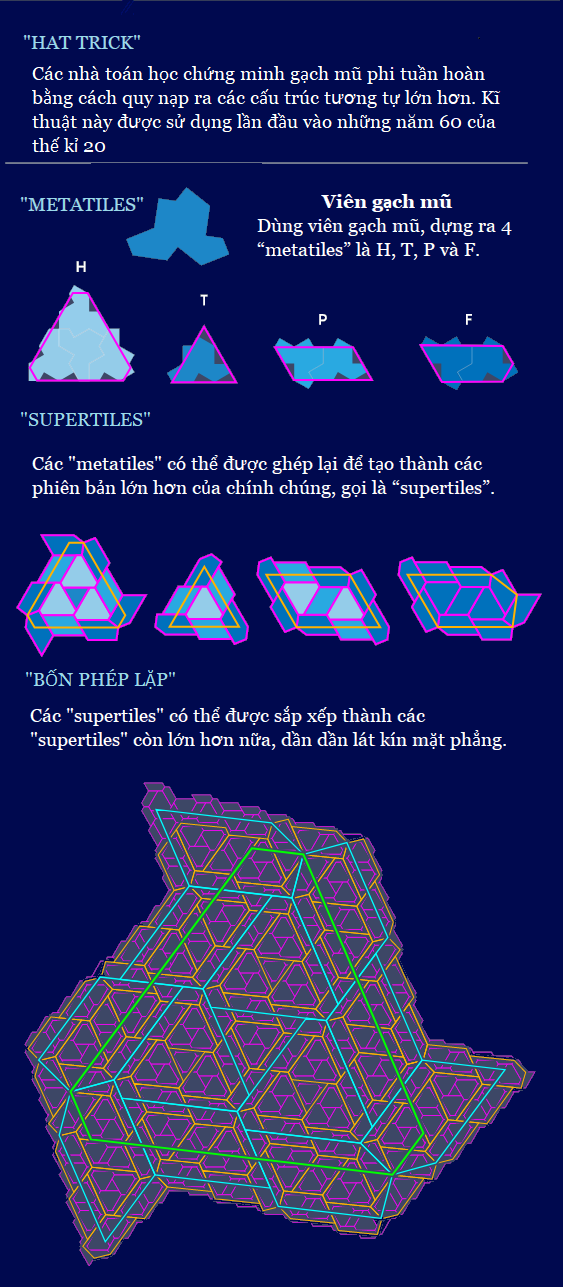
\includegraphics[width= 1\linewidth]{3}
		%		\caption{\small\textit{\color{}}}
		\vspace*{-20pt}
	\end{figure}
	Chứng minh này được biến tấu từ một phương pháp của Berger vào những năm $1960$. Phương pháp đó bao gồm việc ghép một số viên gạch lại với nhau, tạo thành những phiên bản lớn hơn của chính chúng, hình thành một cấu trúc phân chia đẳng cấp. Đầu tiên, Myers xác định bốn hình trung gian được tạo từ viên gạch mũ, gọi là $H$, $T$, $P$ và $F$. Ví dụ, viên gạch $H$ được tạo ra từ $4$ viên gạch mũ, ghép lại thành một hình hao hao một tam giác cụt ở các góc. Myers chứng minh rằng có thể ghép $4$ hình lại với nhau để tạo ra vẫn $4$ hình đó với kích thước lớn hơn. Chẳng hạn, có thể tạo ra một viên gạch $H$ lớn bằng cách xếp ba viên gạch $H$ quanh một viên gạch $T$, rồi ghép các viên gạch $P$ và $F$ xung quanh hình vừa tạo.
	\vskip 0.1cm
	Phương pháp này giúp ta dựng ra những viên gạch lớn dần. Có thể bắt đầu với bất kỳ loại gạch nào, chẳng hạn như viên gạch $H$, phóng to nó lên, và lấp đầy các khe hở  bằng $4$ hình trung gian $H$, $T$, $P$, $F$. Ta có thể lặp đi lặp lại việc này vô số lần để tạo ra một cấu trúc phân cấp từ những hình này, từ đó lát kín mặt phẳng. Đơn vị cơ bản của cấu trúc chính là những viên gạch mũ. 
	\vskip 0.1cm
	Họ đã chứng minh được cách lát hình thành từ các cấu trúc phân cấp này không bao giờ tuần hoàn. Đồng thời họ cũng chỉ ra rằng đó là cách duy nhất để phủ mặt phẳng bằng các hình mũ. Vì thế nên cách phủ mặt phẳng bằng các viên gạch mũ không thể tuần hoàn. ``Một kết quả rất tuyệt vời", Socolar cho hay.
	\vskip 0.1cm
	Vậy là còn lại loại gạch lát thứ hai Smith phát hiện: con rùa. Liệu chăng việc một người đàn ông khám phá ra tận hai loại lát gạch phi tuần hoàn cùng lúc, trong khi phần còn lại của nhân loại bó tay trong suốt 50 năm, đơn thuần là một sự trùng hợp tuyệt diệu? Viên gạch mũ và ``con rùa" nhìn giống nhau đến bất ngờ, khiến các nhà nghiên cứu nghi ngờ rằng con rùa cũng là một viên gạch phi tuần hoàn. Nhưng nghi ngờ vẫn chỉ là nghi ngờ, không phải chứng minh.
	\vskip 0.1cm
	Thế rồi Myers có một khám phá: hóa ra, cả cái mũ và con rùa đều thuộc về một họ gồm vô số viên gạch lát mặt phẳng theo cùng một cách.
	\vskip 0.1cm
	Mỗi viên gạch mũ có $13$ cạnh: $6$ dài, $6$ ngắn tương ứng với các cạnh hình cánh diều, cộng với một cạnh ghép từ hai cạnh cánh diều ngắn. Bằng cách thay đổi kích cỡ độ dài các cạnh của viên gạch mũ, ta có thể thu được vô hạn không đếm được các viên gạch phi tuần hoàn. Tưởng tượng một thanh trượt: di sang trái khiến cạnh ngắn (cùng với một cạnh ghép kể trên) ngắn đi; di sang phải thì cạnh dài nhỏ lại. ``Con rùa" nằm về bên phải so với viên gạch mũ, nhưng đồng thời cũng có vô số hình khác thuộc kiểu tương tự.
	\vskip 0.1cm
	Nếu ta đẩy thanh trượt hết nấc về bên trái, cạnh ngắn sẽ biến mất, viên gạch lúc này có hình chữ $V$ $6$ cạnh;  đẩy hết nấc sang phải thì cạnh dài biến mất và ta được một hình bảy cạnh được đặt tên là ``sao chổi".  Khác với viên gạch mũ, gạch hình chữ $V$ và hình sao chổi có thể được dùng để lát mặt phẳng một cách tuần hoàn. Hình ở trung tâm thanh trượt, tức cạnh dài và cạnh ngắn bằng nhau, cũng có tính chất này.
	\begin{figure}[H]
		\vspace*{-5pt}
		\centering
		\captionsetup{labelformat= empty, justification=centering}
		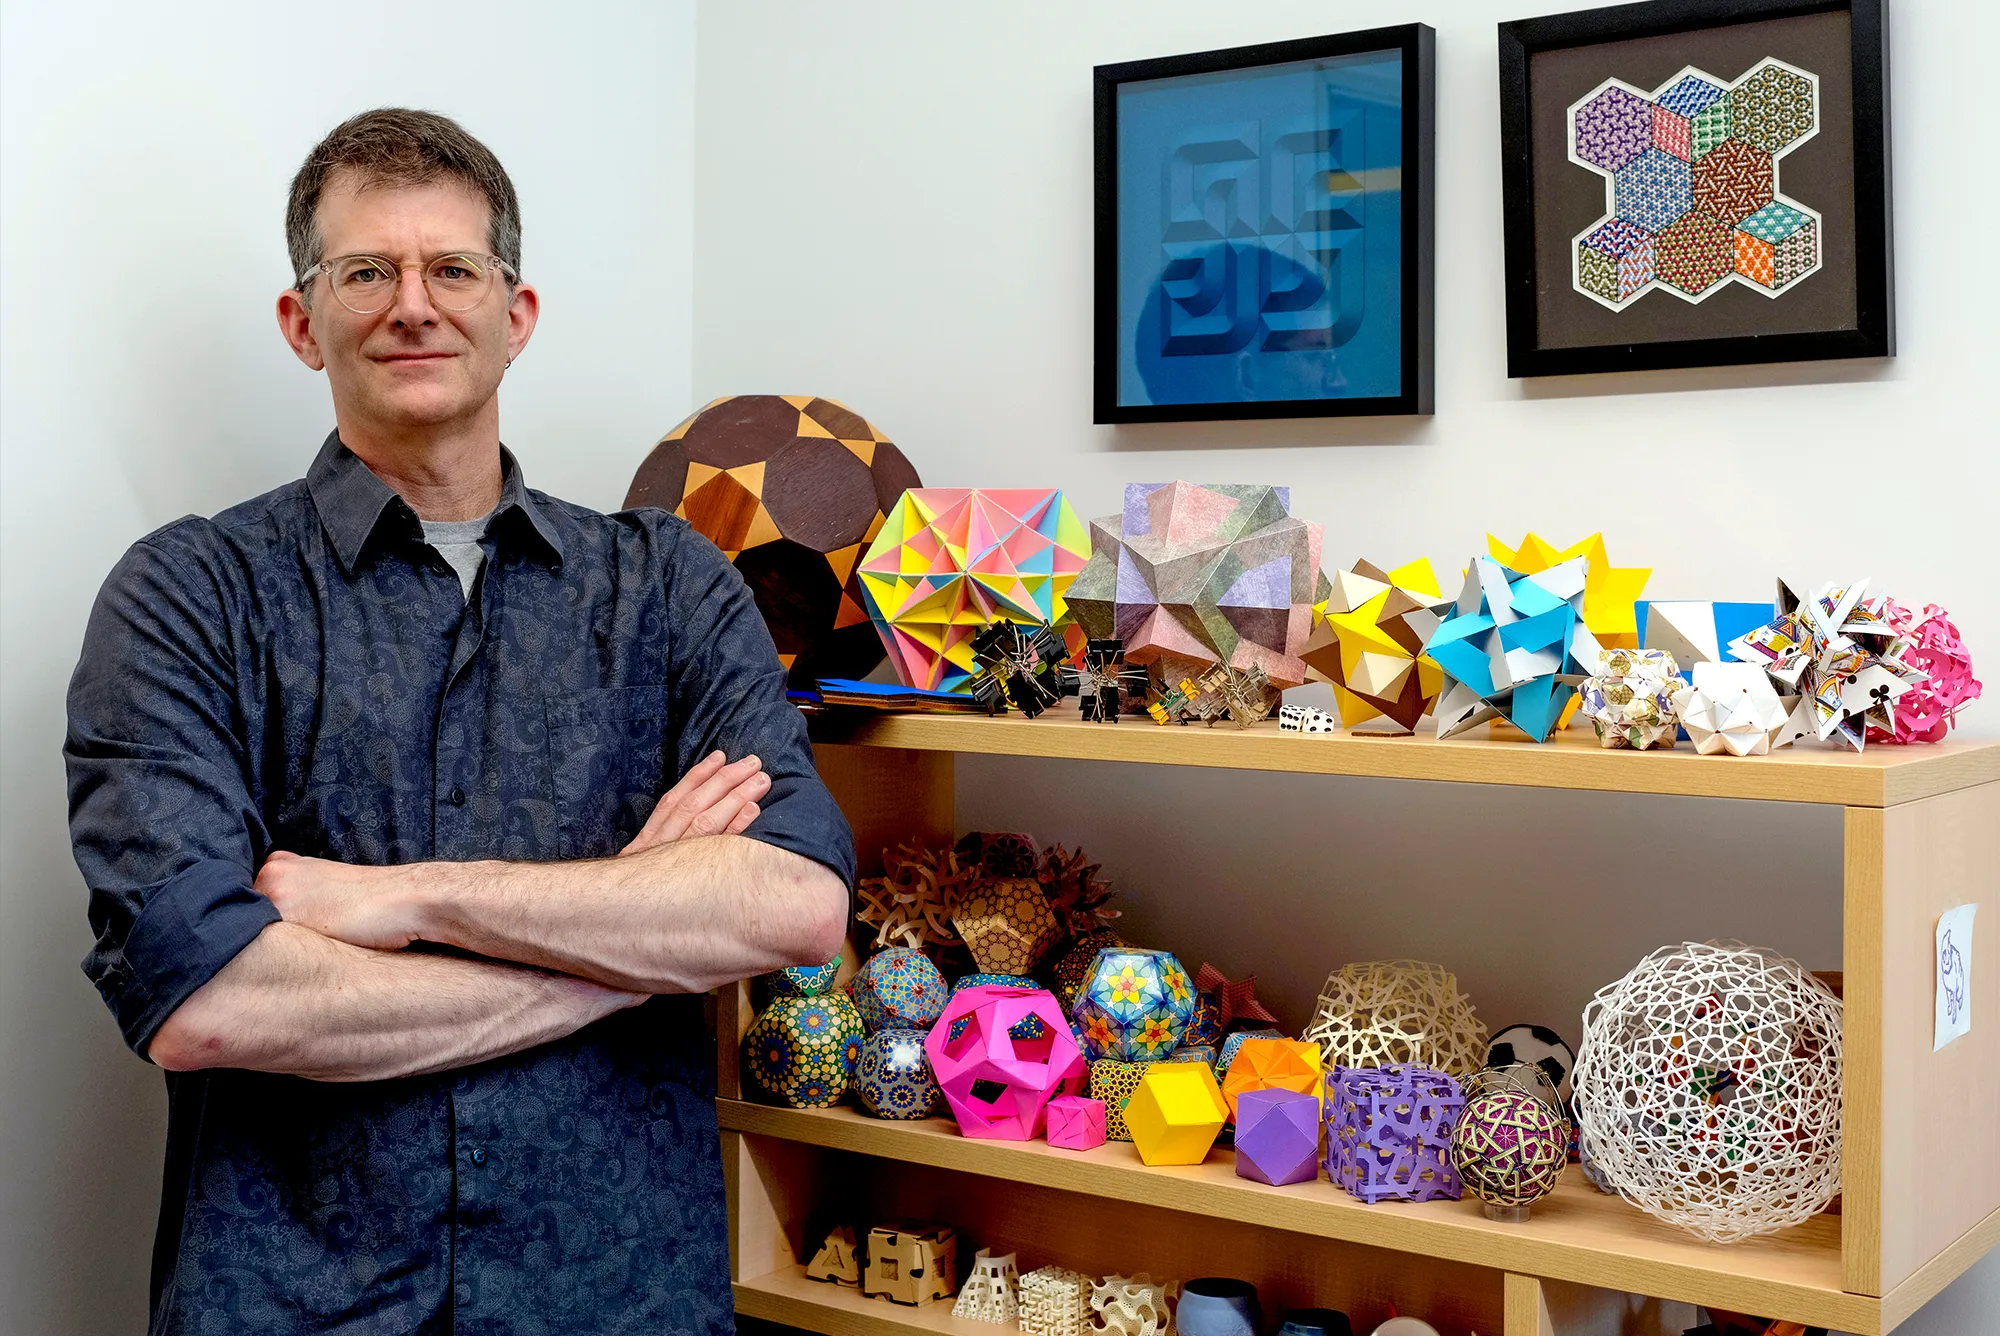
\includegraphics[width= 1\linewidth]{6}
		\caption{\small\textit{\color{duongvaotoanhoc}Craig Kaplan, nhà khoa học máy tính ở đại học Waterloo, Canada.}}
		\vspace*{-10pt}
	\end{figure}
	Myers còn nhận ra rằng mình có thể sử dụng đặc tính hình học của viên gạch chữ $V$ và sao chổi để chứng minh là tất cả các hình dọc theo thanh trượt, trừ hai đầu và trung điểm, đều là gạch loại phi tuần hoàn. Lập luận này, được Kaplan gọi là ``một nước đi thiên tài của Toán học", hoàn toàn mới lạ với bộ môn lát gạch. Trước đây, lĩnh vực này chỉ có $3$ cách tiếp cận chính để chứng minh tính phi tuần hoàn, theo lời Goodman-Strauss. ``Giờ ta có cách thứ tư." 
	\vskip 0.1cm
	Các nhà toán học đang cố gắng thấm phương pháp chứng minh mới này. ``Tôi phải ngồi lại và nghiêm túc dành thời gian cho thứ này," Senechal nói. 
	\vskip 0.1cm
	Một câu hỏi tự nhiên, Greenfield nói, là liệu rằng có thể tìm được một nguồn nào đó tạo ra các cách lát mới không. Năm $1981$, Nicholaas de Brujin [$20$] đã chứng minh được các cách lát Penrose là hình chiếu xuống không gian $2$ chiều của các viên gạch lát tuần hoàn mặt phẳng $5$ chiều. ``Nếu tương tác hoặc cấu trúc của những cách lát (mới) này tương ứng với một cách lát gạch tuần hoàn trên không gian nhiều chiều hơn, điều ấy sẽ thực sự thú vị để tìm hiểu." Greenfield nói.
	\vskip 0.1cm
	Với tư cách một nhà vật lý, Socolar đã bắt đầu khám phá tính chất vật liệu của cách lát mới này. Ông thấy rằng: kiểu nhiễu xạ khi ánh sáng chiếu qua loại gạch lát này có những đỉnh dốc tương tự như ở giả tinh thế. Kể cả khi ấy, cách lát bằng gạch hình mũ vẫn ``trông khác hẳn với tất cả những thứ tôi từng thấy trước đây", ông khẳng định.
	\vskip 0.1cm
	Trong lúc ấy, Smith chưa xong việc với viên gạch ranh mãnh của ông. Ông hiện dự định khám phá tiềm năng nghệ thuật và cách phối màu để làm nổi bật họa tiết của các viên gạch này. ``Dường như nó có thái độ riêng," ông nói. ``Tôi nghĩ ta nên tôn trọng khi làm việc với nó."
	\vskip 0.1cm
	Bình luận của các dịch giả: Có ý kiến cho rằng cái mũ chưa thể được tính là ``einstein" do thực chất chúng ta cần dùng tới cả cái mũ và viên gạch đối xứng trục với nó để lát toàn mặt phẳng, và hai viên gạch có thể tính là khác nhau. Tuy nhiên, đúng như lời hứa, David Smith đã có một phát hiện mới: một trong các họ hàng đặc biệt của cái mũ, gọi là Tile($1, 1$), có thể lát mặt phẳng một cách phi tuần hoàn nếu như ta cấm úp ngược viên gạch lại để ghép. Bằng cách điều chỉnh các cạnh của Tile($1, 1$), ông thu được một họ các viên gạch gọi là bóng ma. Lần này, mỗi bóng ma đều tự nó lát được mặt phẳng phi tuần hoàn, kể cả khi cho phép úp ngược viên gạch này để ghép. Bài báo về phát hiện này [$21$] được đăng lên arXiv vào cuối tháng $5$ năm $2023$, tại thời điểm đăng bài hiện chúng tôi chưa rõ tính xác thực.
	\vskip 0.1cm
	\textbf{\color{duongvaotoanhoc}Các liên kết trong bài viết}
	\vskip 0.1cm 
	[$1$] https://the-orangery.weebly.com/
	\vskip 0.1cm
	[$2$] https://www.jaapsch.net/puzzles/polysol\\
	ver.htm
	\vskip 0.1cm
	[$3$] https://cs.uwaterloo.ca/~csk/
	\vskip 0.1cm
	[$4$] https://arxiv.org/abs/2303.10798
	\vskip 0.1cm
	[$5$] https://www.ams.org/books/memo/00\\
	66/
	\vskip 0.1cm
	[$6$] https://www.engineering.iastate.edu/peo\\
	ple/profile/dannys/
	\vskip 0.1cm
	[$7$] https://link.springer.com/article/10.1007/\\
	BF00239998
	\vskip 0.1cm
	[$8$] http://taylortiling.com/
	\vskip 0.1cm
	[$9$] https://sfb701.math.uni-bielefeld.de/prep\\
	rints/sfb10015.pdf
	\vskip 0.1cm
	[$10$] https://scholars.duke.edu/person/socolar
	\vskip 0.1cm
	[$11$] https://arxiv.org/abs/1003.4279v2
	\vskip 0.1cm
	[$12$] https://www.math.ias.edu/~rgreenfeld/
	\vskip 0.1cm
	[$13$] https://www.math.ucla.edu/~tao/
	\vskip 0.1cm
	[$14$]https://www.quantamagazine.org/nasty-geometry-breaks-decades-old-tiling-conjectur\\
	e-20221215/
	\vskip 0.1cm
	[$15$] http://www.science.smith.edu/~senechal/
	\vskip 0.1cm
	[$16$] https://link.springer.com/article/10.1007\\
	/BF02985414
	\vskip 0.1cm
	[$17$] https://www.quantamagazine.org/marjo\\
	rie-rices-secret-pentagons-20170711/
	\vskip 0.1cm
	[$18$]https://fulbright.uark.edu/departments/\\
	math/directory/index/uid/strauss/name/Chai\\m+Goodman-strauss/
	\vskip 0.1cm
	[$19$] https://www.polyomino.org.uk/
	\vskip 0.1cm
	[$20$] https://www.sciencedirect.com/science/\\
	article/pii/1385725881900172?via\%3Dihub
	\vskip 0.1cm
	[$21$]
	https://arxiv.org/abs/2305.17743
\end{multicols}